\section{Evaluation + Results}

\begin{frame}
    \bigcenter{Evaluation}
\end{frame}

\begin{frame}
    \bigcenter{RQ: Can test results match results of manual grading?}
\end{frame}

\begin{frame}\frametitle{Evaluation, Test Results}
    Test subjects:
    \begin{itemize}
        \item \textcolor{upfim}{37 student implementations} of a simple catching game
        \item from a 6th and 7th grade Scratch workshop~\cite{keller}
        \item \textcolor{upfim}{Graded manually}, on a scale from 0 to 30
    \end{itemize}

    \pause
    \bigskip

    Two test suites:
    \begin{itemize}
        \item \textcolor{upfim}{''normal'' test suite} with 28 test cases
            \begin{itemize}
                \item each test case executes the program once, independently
            \end{itemize}
        \item \textcolor{upfim}{''constraint'' test suite} with 26 constraints
            \begin{itemize}
                \item only one test case
                \item uses generated input
                \item runs the program for 10s with 30 resets $\rightarrow$ 300s
            \end{itemize}
    \end{itemize}

    \pause
    \bigskip

    Measured item:
    \begin{itemize}
        \item \textcolor{upfim}{Correlation} between manual scores and the number of test or constraint passes
    \end{itemize}
\end{frame}

\begin{frame}\frametitle{Evaluation, Test Results}
    Excluded Projects:
    \begin{itemize}
        \item 6 of the 37 projects were excluded from the calculation
        \item Most because they don't start with the \greenflag event, but with other key presses
            \begin{itemize}
                \item Tests try to start the program with the \greenflag button
                \item Not an issue for manual grading
            \end{itemize}
    \end{itemize}

    % TODO: note the excluded projects for potential questions
\end{frame}

\begin{frame}\frametitle{Evaluation, Test Results, Normal Tests}
    \begin{figure}
        \begin{minipage}{.85\textwidth}
            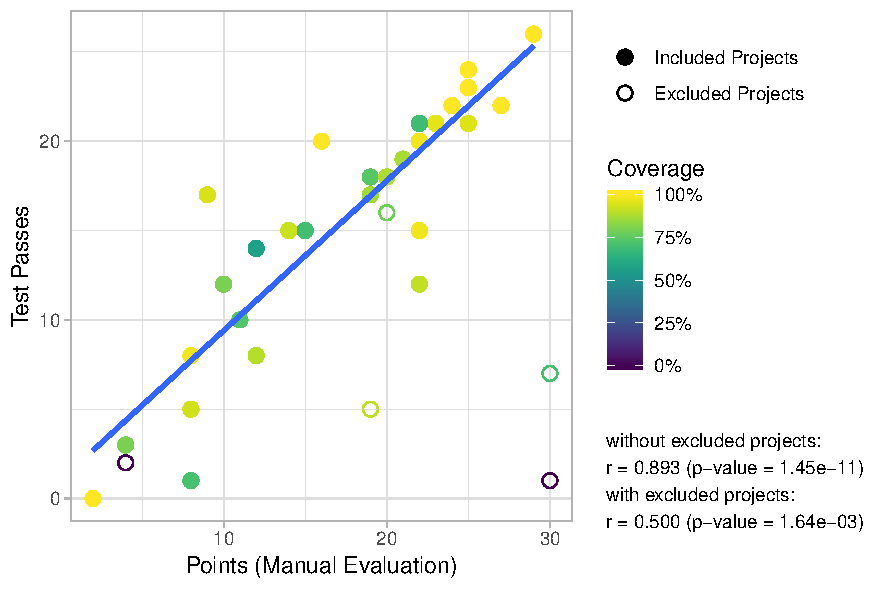
\includegraphics[width=\textwidth]{r/scatter-normal-1}
            \caption{Comparison between results of normal tests and manual scores, 1st run}
        \end{minipage}
    \end{figure}
\end{frame}

\begin{frame}\frametitle{Evaluation, Test Results, Normal Tests}
    \begin{figure}
        \begin{minipage}{.85\textwidth}
            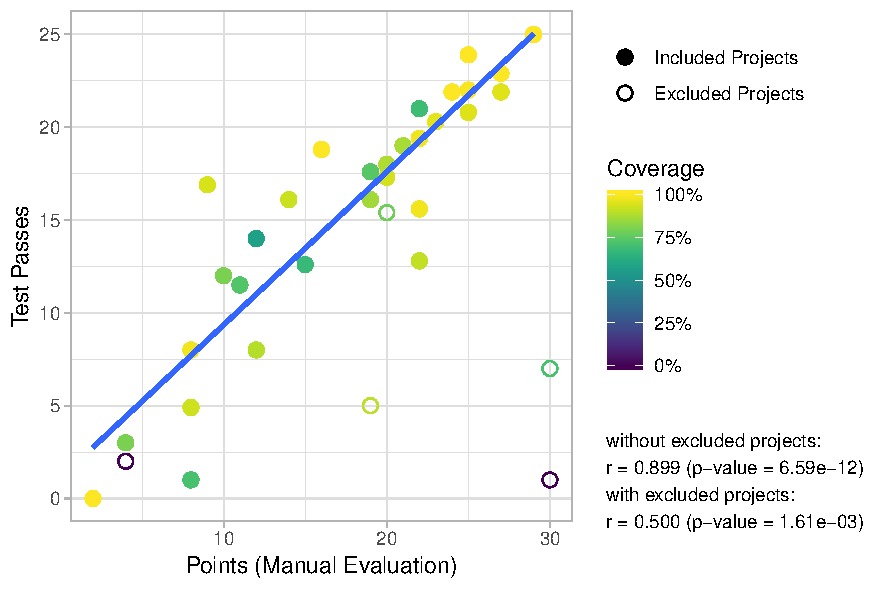
\includegraphics[width=\textwidth]{r/scatter-normal-avg}
            \caption{Comparison between results of normal tests and manual scores, average over 10 runs}
        \end{minipage}
    \end{figure}
\end{frame}

\begin{frame}\frametitle{Evaluation, Test Results, Constraint Tests}
    \begin{figure}
        \begin{minipage}{.85\textwidth}
            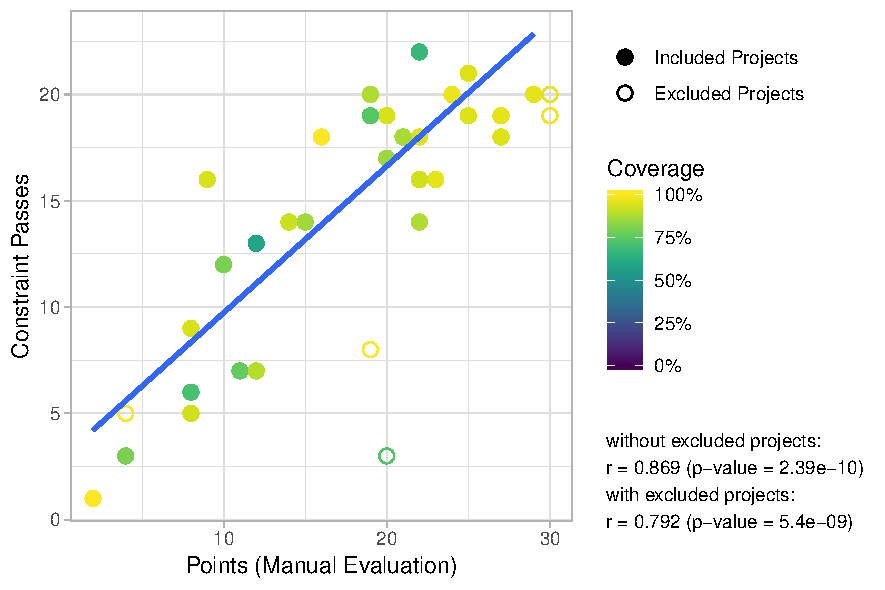
\includegraphics[width=\textwidth]{r/scatter-random-1}
            \caption{Comparison between results of constraint tests and manual scores, 1st run}
        \end{minipage}
    \end{figure}
\end{frame}

\begin{frame}\frametitle{Evaluation, Test Results, Constraint Tests}
    \begin{figure}
        \begin{minipage}{.85\textwidth}
            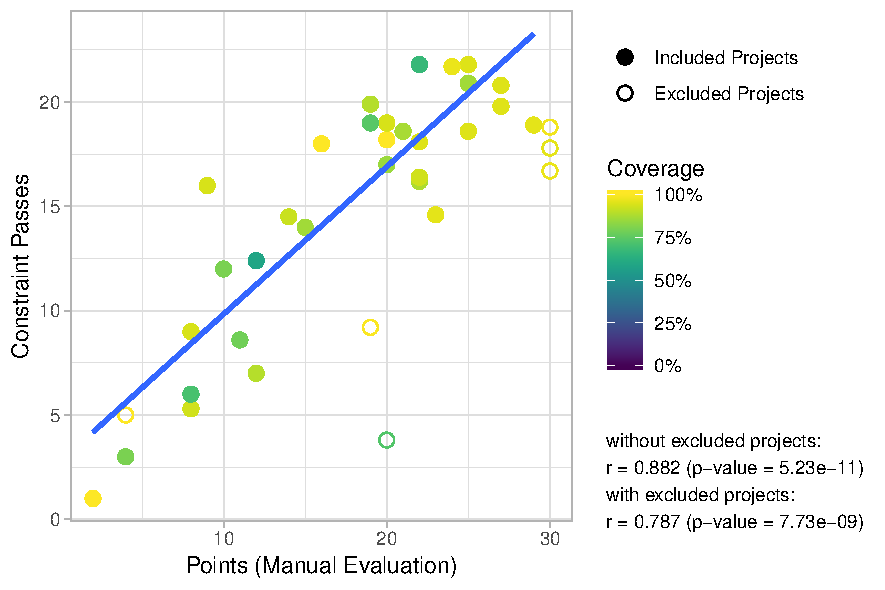
\includegraphics[width=\textwidth]{r/scatter-random-avg}
            \caption{Comparison between results of constraint tests and manual scores, average over 10 runs}
        \end{minipage}
    \end{figure}
\end{frame}

\begin{frame}
    \bigcenter{RQ: What coverage can be achieved with automated input?}
\end{frame}

\begin{frame}\frametitle{Evaluation, Coverage of Automated Input}
    Test subjects:
    \begin{itemize}
        \item 24 sample solutions to Code Club's\footnote{\url{https://codeclubprojects.org/}} online Scratch courses
        \item Run with generated input for 10 minutes
    \end{itemize}

    \pause
    \bigskip

    Measured item:
    \begin{itemize}
        \item Mean coverage of the projects after 10 minutes
        \item Coverage measured every second
    \end{itemize}
\end{frame}

\begin{frame}\frametitle{Evaluation, Coverage of Automated Input}
    \begin{figure}
        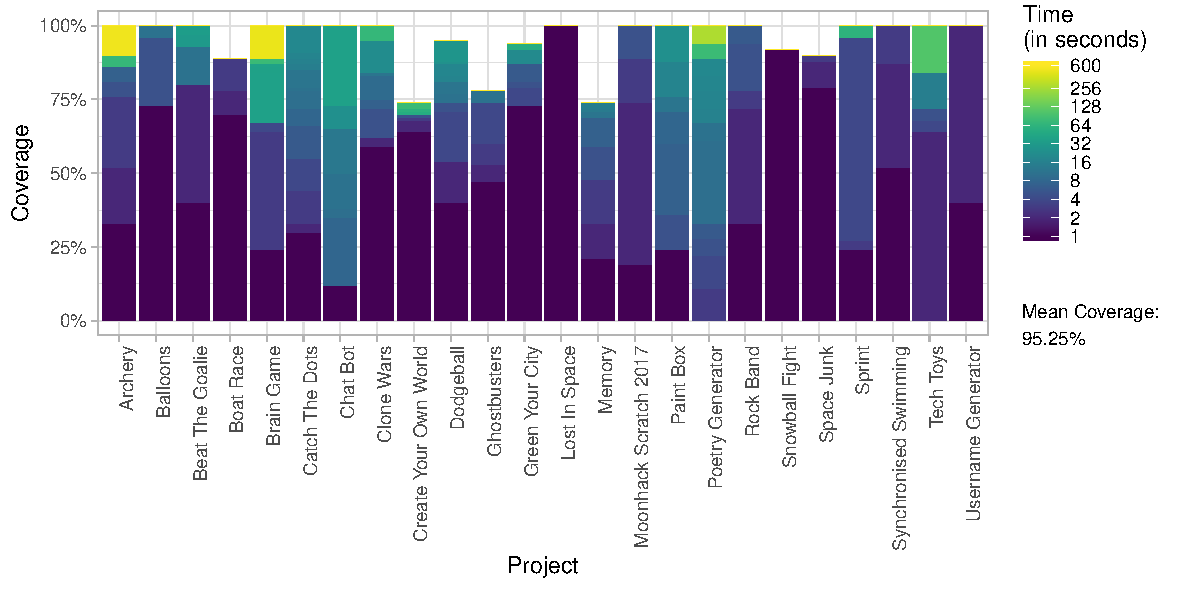
\includegraphics[width=\textwidth]{r/coverage-bar-random-input-1}
        \caption{Coverage per project, 1st run}
    \end{figure}
\end{frame}

\begin{frame}\frametitle{Evaluation, Coverage of Automated Input}
    \begin{figure}
        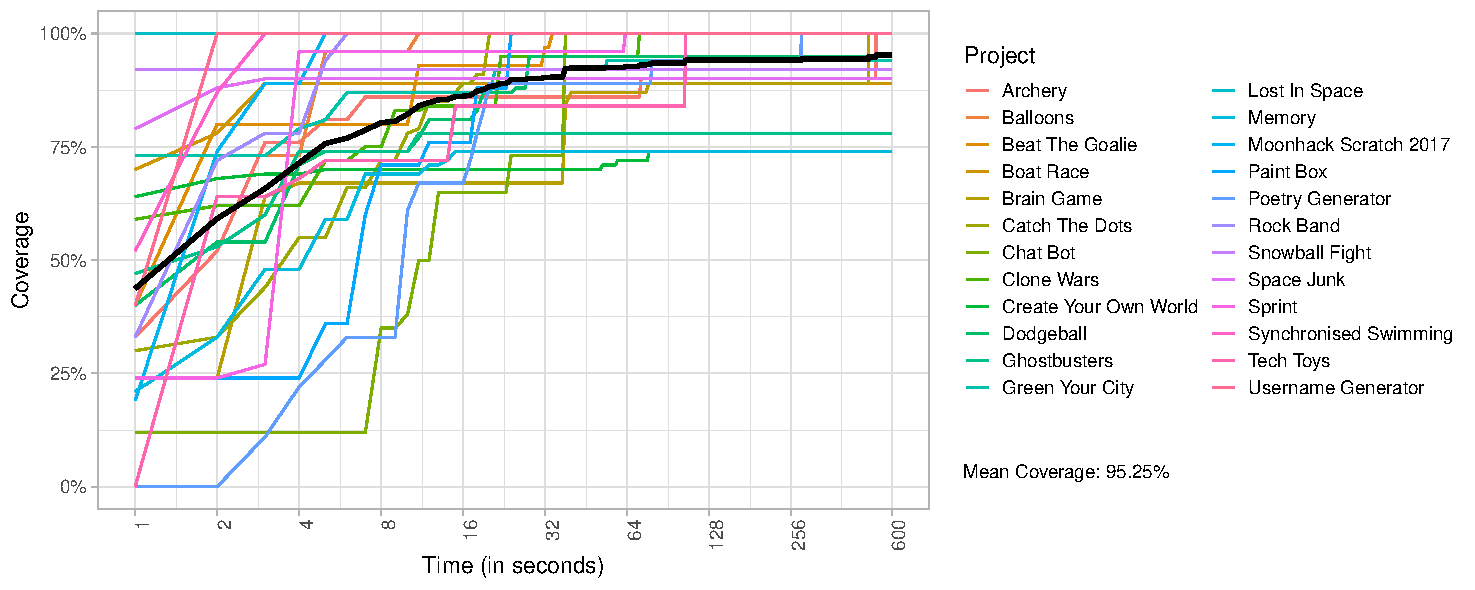
\includegraphics[width=\textwidth]{r/coverage-line-random-input-1}
        \caption{Coverage over time, 1st run}
    \end{figure}
\end{frame}

\begin{frame}\frametitle{Evaluation, Coverage of Automated Input}
    \begin{figure}
        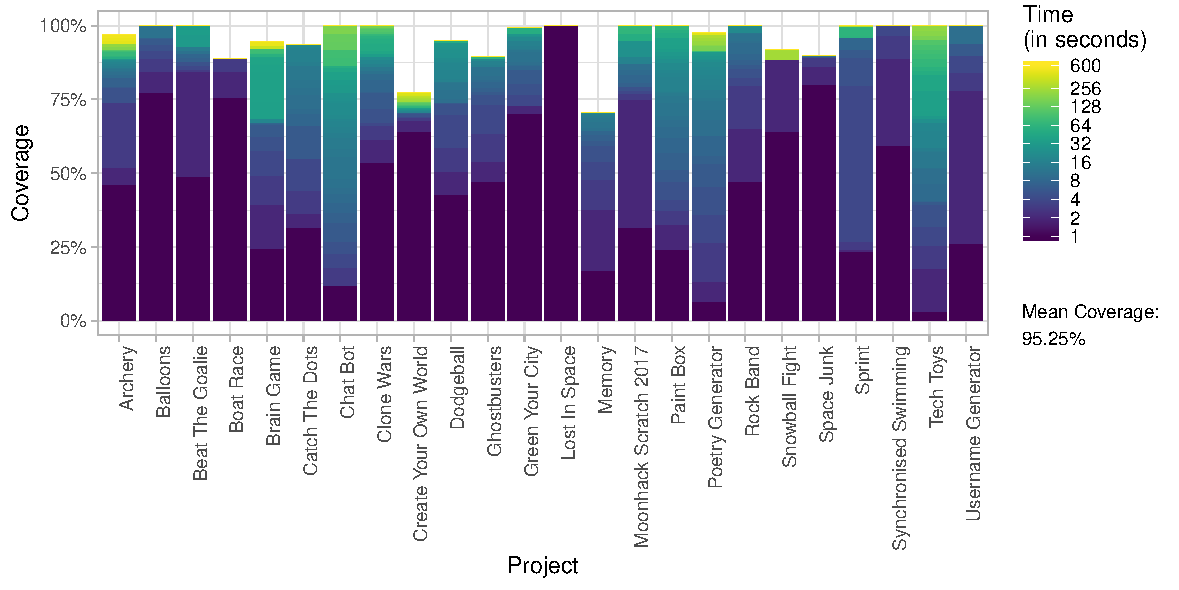
\includegraphics[width=\textwidth]{r/coverage-bar-random-input-avg}
        \caption{Coverage per project, average over 10 runs}
    \end{figure}
\end{frame}

\begin{frame}\frametitle{Evaluation, Coverage of Automated Input}
    \begin{figure}
        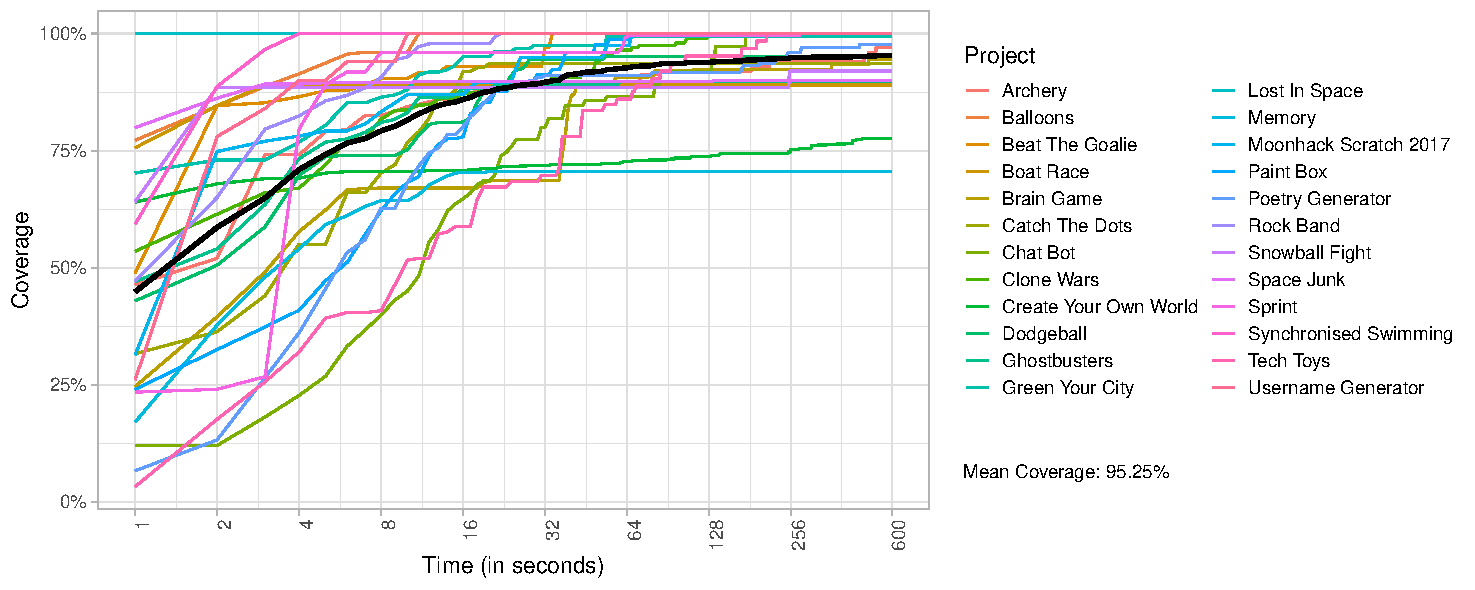
\includegraphics[width=\textwidth]{r/coverage-line-random-input-avg}
        \caption{Coverage over time, average over 10 runs}
    \end{figure}
\end{frame}

\begin{frame}\frametitle{Evaluation, Coverage of Automated Input}
    \begin{figure}
        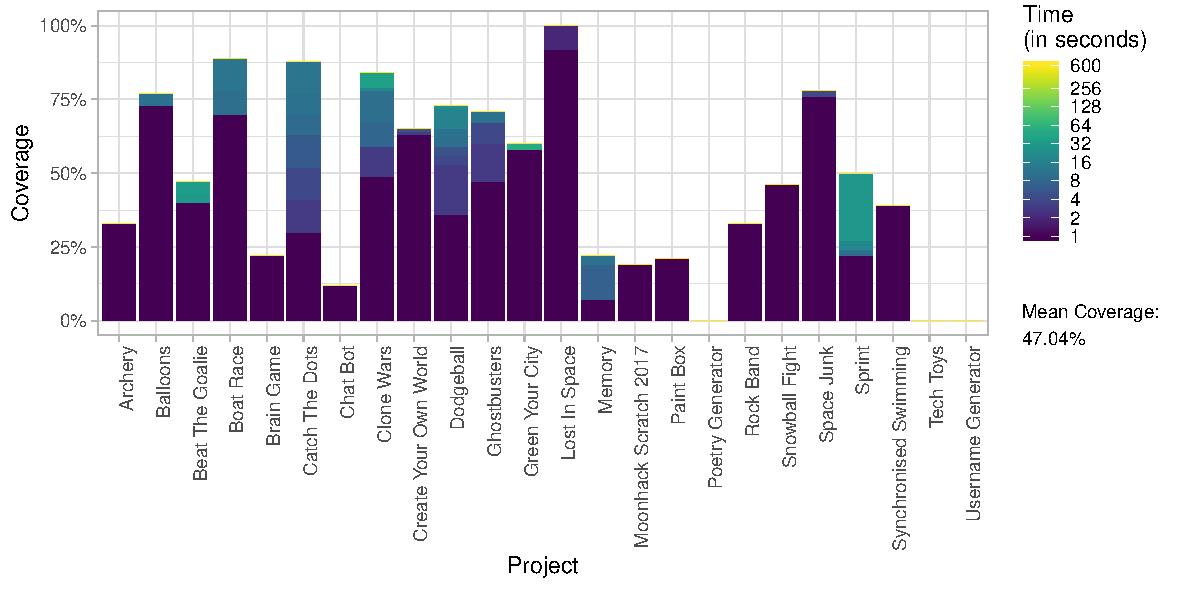
\includegraphics[width=\textwidth]{r/coverage-bar-no-input-1}
        \caption{Coverage per project, 1st run}
    \end{figure}
\end{frame}

\begin{frame}\frametitle{Evaluation, Coverage of Automated Input}
    \begin{figure}
        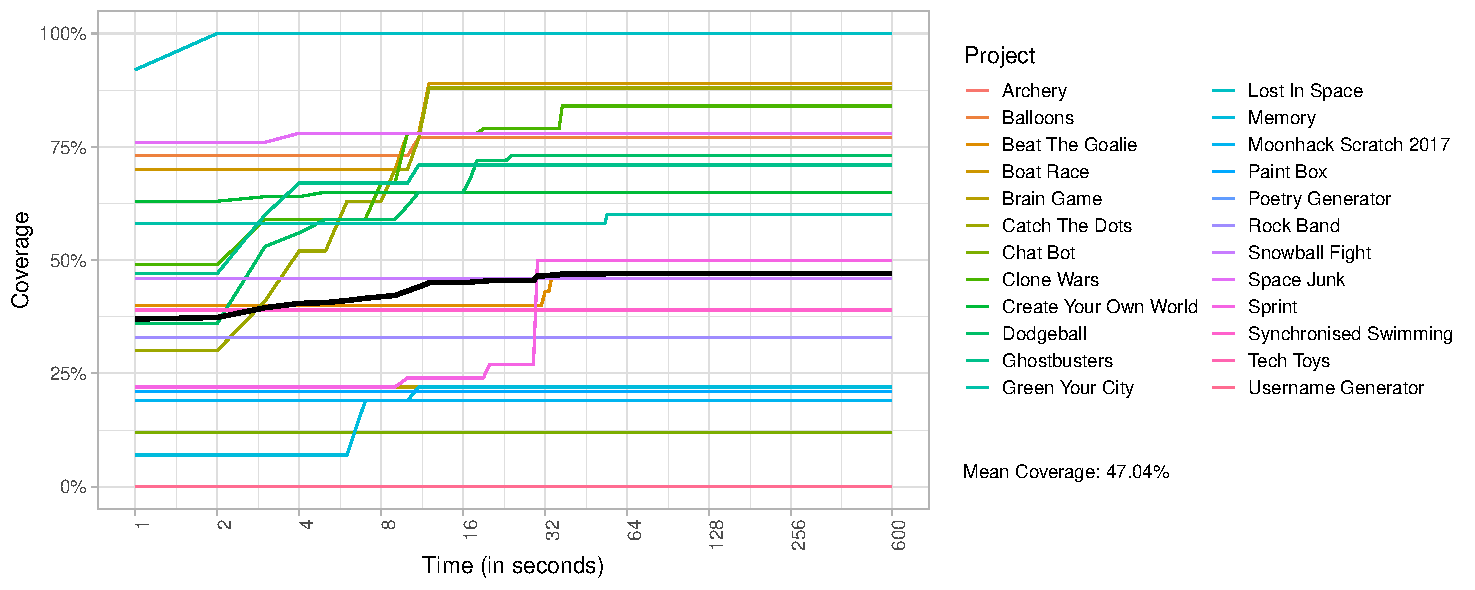
\includegraphics[width=\textwidth]{r/coverage-line-no-input-1}
        \caption{Coverage over time, 1st run}
    \end{figure}
\end{frame}

\begin{frame}\frametitle{Evaluation, Coverage of Automated Input}
    \begin{figure}
        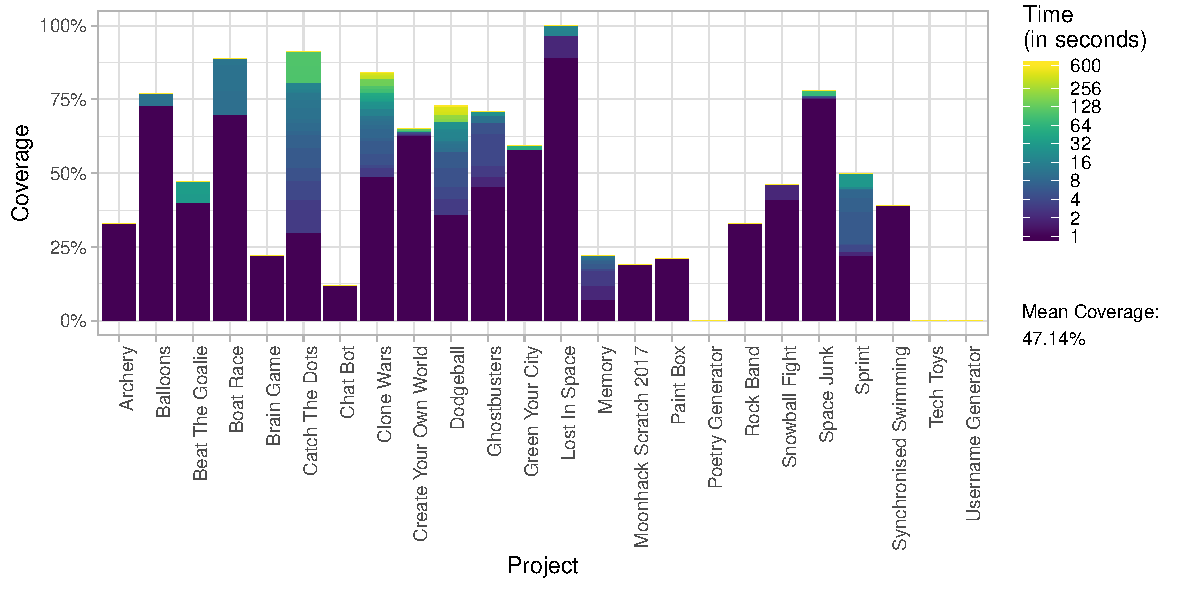
\includegraphics[width=\textwidth]{r/coverage-bar-no-input-avg}
        \caption{Coverage per project, average over 10 runs}
    \end{figure}
\end{frame}

\begin{frame}\frametitle{Evaluation, Coverage of Automated Input}
    \begin{figure}
        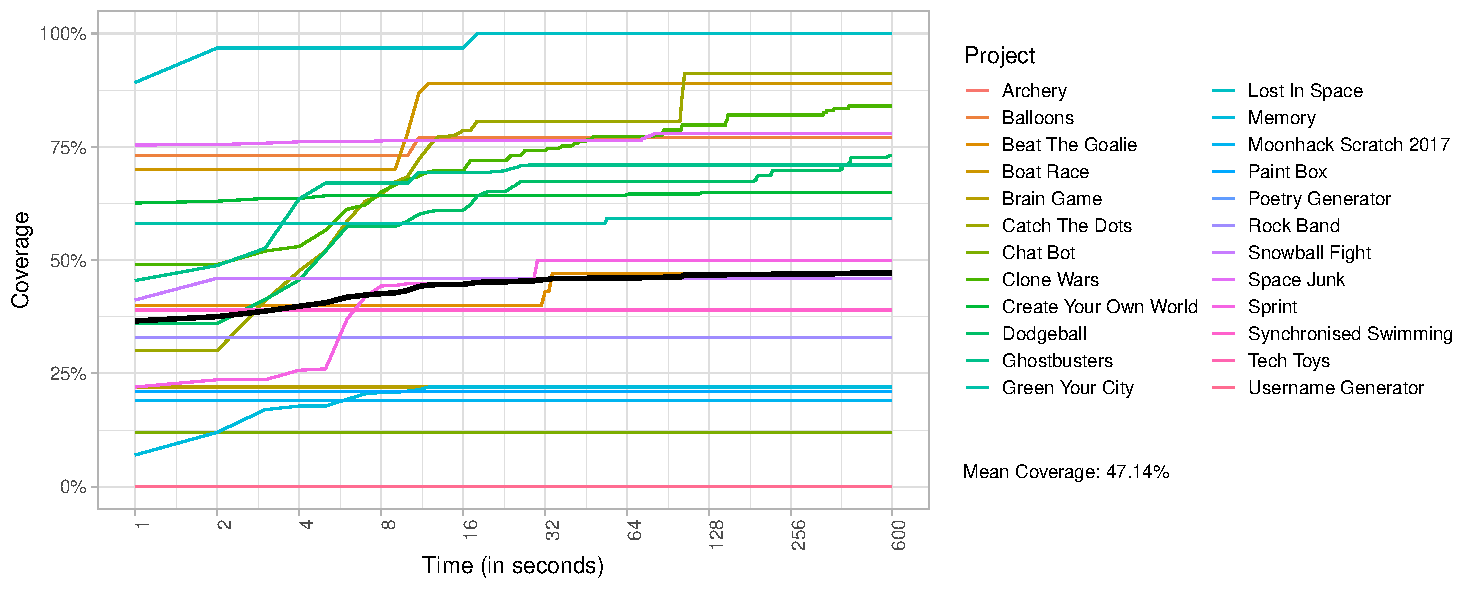
\includegraphics[width=\textwidth]{r/coverage-line-no-input-avg}
        \caption{Coverage over time, average over 10 runs}
    \end{figure}
\end{frame}
